% !TeX root = ../main.tex
% Add the above to each chapter to make compiling the PDF easier in some editors.

\chapter{Design}\label{chapter:design}
\section{Trust, Usability and Privacy}
To create a platform that both produces useful data while protecting the privacy of their creator, we have to find a balance between usability and privacy. It is not an easy task to achieve both because often these two are opposites of each other. However, another aspect that influences both is trust. Data that can not be trusted is useless, and services that are not trustworthy should not be allowed with privacy relevant tasks.
 
In any platform, we expect a certain level of trust from each participant, may it be from the service provider or its consumer. How this trust is created can have many different sources. Nevertheless, the main reason a person or organization can be trusted is because of accountability. Companies with a strong market presence have the public's trust since they have been present for a more extended period and can not just disappear overnight
 Consequently, they can be held accountable for their actions. Today, Microsoft, Google, Amazon, and Facebook, for instance, are seen as trustworthy to a certain degree. However, this trust is not invulnerable. Lies and secrecy can damage trust. Keeping the public uninformed about severe data breaches or selling sensitive data to third parties without their knowledge and permission has strained the public trust in recent years.

As chapter 2 has shown, it is a hard task to anonymize big data sets, as we can use quasi-identifiers to infer new information using linking attacks. So one way to achieve anonymity would be to strip away all attributes that are available in another data set. Here we hit an obstacle with the usability of the data itself. Cynthia Dwork \cite{dwork} says, "de-identified data isn't," meaning that either that the data itself can be re-identified because of possible reconstruction of the data or it is not data anymore because it is not useful for analysis purposes. We see data only as useful as its relationships.

It is necessary to find a way to balance trust, usability, and privacy. However, due to the limited scope of our thesis, we mainly focus on privacy and usability. We assume that all participating devices and servers can be trusted, and possible adversaries only have access to the published end results.

\section{Approaches}
As mentioned in the beginning, there are advantages and disadvantages to van Endern's \cite{simon} system, and we explore how we can implement improvements and if they would be feasible with the current state of the art or if we have to choose another alternative.

\subsection{Simon van Endern's Approach}
The proposed architecture implemented in his thesis was using a centralized program with a distributed storage solution. The model can be seen in Figure \ref{fig:simon_original}.

\begin{figure}[htpb]
  \centering
  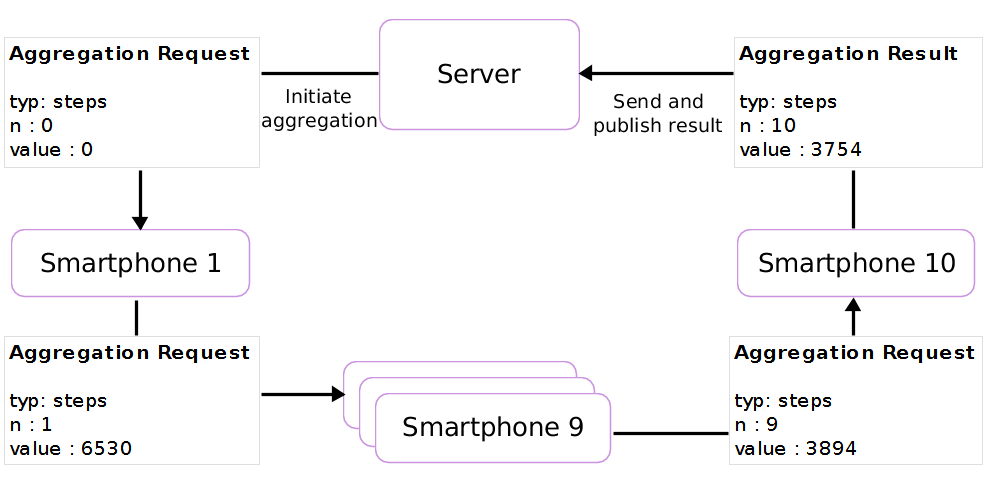
\includegraphics[width=0.8\textwidth]{figures/simon_original.png}
  \caption{Simon van Endern's original architecture \cite{simon}} \label{fig:simon_original}
\end{figure}

In his work, he eliminates the need for a central database, by collecting and storing raw data directly on the users' smartphone, creating kind of a distributed database. It gives each participant a lot of control over their data, just by deleting the application or disabling internet connection they can opt-out of future data analyses.

In his original idea, the mobile phones would use peer-to-peer technology to forward the aggregation requests between themselves and finally send the result to the server for publication. Because of the lack of available technology, however, he opted to use the central server as an intermediary to forward requests from mobile phone to mobile phone. To keep the data confidential and ensure anonymity from the server, he uses RSA and AES encryption. To pass on the data to the next device, he implemented a polling solution. Each application periodically asks for a new aggregation request targeted at their device from the server. If one is present, it fetches the request over the REST API, and after adding its data, it posts it back to the server targeting the next device.
In the finite scope, he managed to implement three aggregation types:

\begin{itemize}
    \item Average number of steps over a day for participants. 
    \item Average time spent on an activity (walking, running, in a vehicle or on a bicycle).
    \item Average number of steps of a participant during the test period. 
\end{itemize}

We examined his work and discovered a few flaws that we might be able to refine. We will look into possible solutions to make the architecture more efficient, scalable, secure, and privacy-preserving.

\subsection{Expanded Approach}
Van Endern's original idea, as is, can hardly be scaled because of the nature of its forwarding chain. Adding \(n\) new devices creates a linear time complexity of \(\mathcal{O}(n)\) and space complexity of \(\mathcal{O}(n^2)\). For every device added, the aggregation takes up to an additional 15 minutes, and the data fetched and sent is the combination of all data of the previous devices, making it quite a burden on each participant's data plan depending on their position in the chain.

\subsubsection{Parallelization}
Our first goal is to make the platform more efficient and scalable. We propose to parallelize the chains by building multiple groups for the aggregation, as shown in Figure \ref{fig:ar}. Each chain in itself resembles van Endern's original idea in Figure \ref{fig:simon_original}. With \(m\) groups, adding \(n\) devices, it only creates a time complexity of \(\mathcal{O}(\dfrac{n}{m})\) and space complexity of \(\mathcal{O}((\dfrac{n}{m})^2)\). So dynamically choosing the right \(m\) could change linear and quadratic growth to potentially constant growth. 

\begin{figure}[htbp]
  \centering
  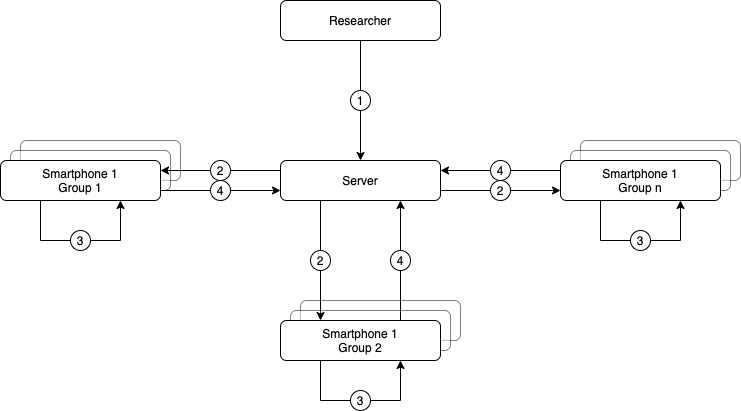
\includegraphics[width=0.8\textwidth]{figures/ar}
  \caption{Data flow of an aggregation in the new architecture} \label{fig:ar}
\end{figure}

\begin{enumerate}
    \item Researcher sends aggregation request to a central server
    \item Server forwards aggregation request to each group
    \item Each group, aggregates the data internally
    \item Finally the last device in each group returns the results to the central server
\end{enumerate}

\subsubsection{Peer-to-Peer}
In the internal aggregation, we leverage the power of peer-to-peer technology to send data directly from one device to the next one without the help of an intermediate third party. In there, each mobile phone receives data from the previous device, adds its own, and then sends it to the next participant, similar to van Endern's idea in Figure \ref{fig:simon_original}.

After research, we found the open-source projects, IPFS \cite{DBLP:journals/corr/Benet14} and libp2p \cite{libp2p}, which are trying to be the new foundation of the decentralized and distributed web of the future. IPFS uses hashes to create content identifiers and turns them into blocks in a directed acyclic graph. To discover the peers storing the content, it uses a distributed hash table, utilizing the modular peer-to-peer networking stack libp2p to communicate directly between nodes.

Built on those technologies, we identify Textile as a promising framework that can help us realize our peer-to-peer connected platform. Their main feature threads is a hash-chain of blocks that can represent any data set, which we could use to send data directly.

After the group aggregation, we have the choice to either combine the data on a final device before sending it to the server for publication or to send them to the server for final aggregation. We choose against the latter because of limited data coverage for mobile devices. Most mobile phone plans have a data cap they are able to use, after which bandwidth is throttled. Keeping this limit in mind, we opted for the collection of the data on the server, sacrificing a little bit of privacy for the deficits of mobile computing.

Another flaw to van Endern's architecture is the constant polling for new aggregation requests. Each user asks for a request targeted at their device and will do so every 15 minutes. Depending on the number of participants, it could mean up to millions of messages to the server every few minutes. Taking advantage of peer-to-peer also solves this problem and cut down on those delays. 

\subsubsection{Additional Aggregation Types}
Besides architectural design changes, we also want to collect more data, especially real location data. In order to extend the aggregation options, we add the following two types:
\begin{itemize}
    \item The location of all participants in a specified area at a specified time
    \item The number of participants in a specified area at a specified time frame
\end{itemize}

\subsubsection{Spatial Cloaking}
To be able to provide k-anonymity for location data, we have to be able to generalize the GPS coordinates. By using spatial cloaking algorithms, we can hide the true position and hide the identifying landmarks by assigning the user to an approximate area. Normally, spatial cloaking algorithms try to minimize the area covered by spanning the cloaked region using the devices as corner points or border points. It, however, would reveal the actual locations of the participants if for k-anonymity k=2. So, we consider using Casper, Interval Cloaking, or Hilbert Cloaking to improve our platform on the privacy-preservation front. 

\subsubsection{Differential Privacy}
We look into the benefits and the disadvantages that the implementation of differential privacy could bring in our design. It is a powerful tool that can guarantee privacy. On the one hand, global differential privacy provides accurate data representation, but the algorithm needs the real values of the data infringing on our privacy-preserving requirement. Local differential privacy, on the other hand, can provide privacy without the intermediate data collector because of its composition feature. A disadvantage that local differential privacy brings is the necessity for a large data set. Since the noise addition to every entry in the set creates a much higher total noise level than global differential privacy and a huge number of participants is needed to cancel that out.

We considered implementing differential privacy, but ultimately decided against it. The global mechanism requires the server to have access to all raw values, while the local approach would add too much noise. In addition, differential private algorithms can currently only applied to simple data schemes, such as sums and counts, which would work with steps, activities, and presence data. However, it can not be applied to location. Also, because of the high sensitivity of the values, because of our lack of participants, we are unable to cancel out the accumulated noise, basically making our collected data useless.
